% Name: Use case diagram
% Description: A customer and a payment provider outside an online shop, the use cases they take part in, and an include and an extend between use cases.
% Tags: use case diagram, UML, actors, requirements

\usetikzlibrary{arrows.meta, shapes.geometric}

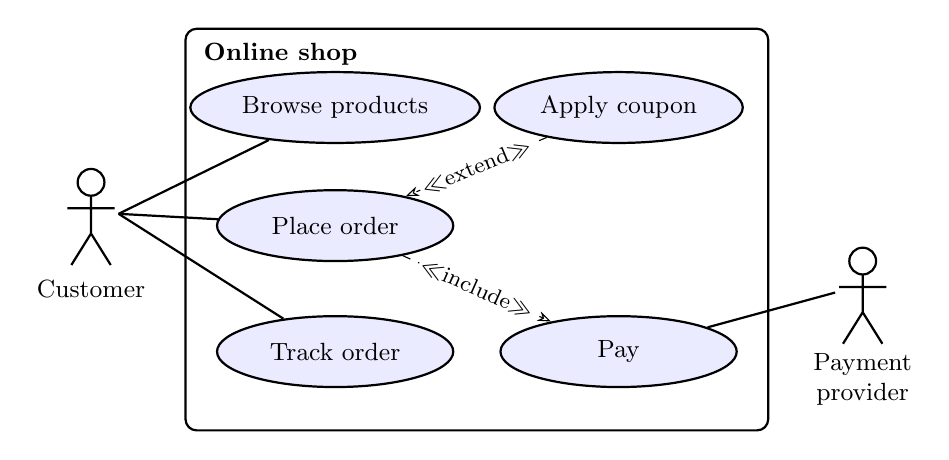
\begin{tikzpicture}[every node/.style={font=\small}, thick,
    usecase/.style={ellipse, draw, fill=blue!8, minimum width=30mm, minimum height=9mm},
    dep/.style={-{Stealth[open]}, dashed, thin},
    actor/.pic={\draw (0,0.55) circle (0.17) (0,0.38) -- (0,-0.1) (-0.3,0.22) -- (0.3,0.22) (-0.25,-0.5) -- (0,-0.1) -- (0.25,-0.5);}]
  \draw[rounded corners] (-0.2,-3.2) rectangle (7.2,1.9);
  \node[anchor=north west, font=\small\bfseries] at (-0.1,1.85) {Online shop};
  \node[usecase] (browse) at (1.7,0.9) {Browse products};
  \node[usecase] (order) at (1.7,-0.6) {Place order};
  \node[usecase] (track) at (1.7,-2.2) {Track order};
  \node[usecase] (pay) at (5.3,-2.2) {Pay};
  \node[usecase] (coupon) at (5.3,0.9) {Apply coupon};
  \pic at (-1.4,-0.6) {actor};
  \node at (-1.4,-1.4) {Customer};
  \pic at (8.4,-1.6) {actor};
  \node[align=center] at (8.4,-2.55) {Payment\\provider};
  \foreach \u in {browse, order, track} \draw (-1.05,-0.45) -- (\u);
  \draw (8.05,-1.45) -- (pay);
  \draw[dep] (order) -- node[sloped, fill=white, inner sep=1pt, font=\footnotesize] {$\ll$include$\gg$} (pay);
  \draw[dep] (coupon) -- node[sloped, fill=white, inner sep=1pt, font=\footnotesize] {$\ll$extend$\gg$} (order);
\end{tikzpicture}
